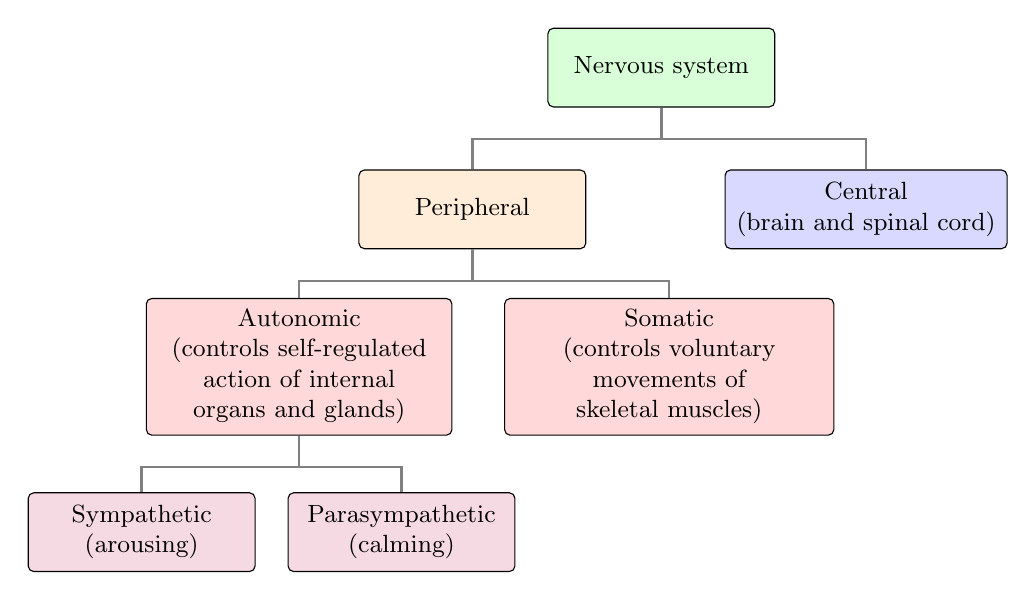
\begin{tikzpicture}[font=\small,
    box/.style={draw, rounded corners=2pt, align=center, minimum height=1.0cm, inner sep=4pt, execute at begin node={\hyphenpenalty=10000}},
    edge/.style={gray, line width=0.9pt}]
  \node[box, fill=green, fill opacity=0.15, text opacity=1, text width=2.6cm] (ns) at (0,0) {Nervous system};
  \node[box, fill=orange, fill opacity=0.15, text opacity=1, text width=2.6cm] (p) at (-2.4,-1.8) {Peripheral};
  \node[box, fill=blue, fill opacity=0.15, text opacity=1, text width=3.3cm] (c) at (2.6,-1.8) {Central\\(brain and spinal cord)};
  \node[box, fill=red, fill opacity=0.15, text opacity=1, text width=3.6cm] (a) at (-4.6,-3.8) {Autonomic\\(controls self-regulated action of internal organs and glands)};
  \node[box, fill=red, fill opacity=0.15, text opacity=1, text width=3.9cm] (s) at (0.1,-3.8) {Somatic\\(controls voluntary movements of skeletal muscles)};
  \node[box, fill=purple, fill opacity=0.15, text opacity=1, text width=2.6cm] (sy) at (-6.6,-5.9) {Sympathetic\\(arousing)};
  \node[box, fill=purple, fill opacity=0.15, text opacity=1, text width=2.6cm] (pa) at (-3.3,-5.9) {Parasympathetic\\(calming)};
  \draw[edge] (ns.south) -- ++(0,-0.4) -| (p.north);
  \draw[edge] (ns.south) -- ++(0,-0.4) -| (c.north);
  \draw[edge] (p.south) -- ++(0,-0.4) -| (a.north);
  \draw[edge] (p.south) -- ++(0,-0.4) -| (s.north);
  \draw[edge] (a.south) -- ++(0,-0.4) -| (sy.north);
  \draw[edge] (a.south) -- ++(0,-0.4) -| (pa.north);
\end{tikzpicture}
